\chapter{Methodology}

This work is following B. Tekin's real-time single shot 6D object pose detection method \cite{tekin2018real} which is inspired by the performance of YOLO \cite{redmon2016you} and YOLO v2 on single shot 2D object detection. The network architecture is based on YOLO v2  but extends 2D detection to 6D detection task. The output of the network is the 2D coordinates of the projections of the 3D keypoints of the object which is then applied to a PnP algorithm to compute the camera pose together with the ground 3D points.

In this section, we first review the network architecture of some single shot object detection methods, we take YOLO and YOLO v2  for examples, and then elaborate our improvements on it for a camera localization problem.

\section{Single shot object detection}

The network architecture of our work is based on YOLO v2 but is amenable to other single shot detectors such as SSD and its variants. In this section we briefly introduce the network architecture of YOLO and YOLO v2.

YOLO \cite{redmon2016you} is a single shot object detection approach which first frames object detection as a regression problem to spatially separated bounding boxes and associated class probabilities, instead of the prior repurposing to classification works.

YOLO uses a single neural network to predict bounding boxes and class probabilities directly from full images in one evaluation. Given an input image, the system divides the image into an $S \times S$ grid. The grid that the center of an object falls into is responsible for detecting that object. Each grid cell predicts B bounding boxes and confidence scores for those boxes. The confidence score reflects how confident the model is that the box contains an object and also how accurate it thinks the box that it predicts is. YOLO takes the intersection over union (IOU) as the measurements for the confidence score. Formally, the confidence is defined as $Pr(Object) * IOU_{pred}^{truth}$. That is, if no object exists in the cell, the confidence is 0. Otherwise the confidence score equals the intersection over union (IOU) between the predicted box and the ground truth. Each grid cell also predicts C conditional class probabilities, $Pr(Class_{i}|Object)$. These probabilities are conditioned on the grid cell containing an object. There is only one set of class probabilities predicted per grid cell, regardless the number of bounding boxes B is predicted per cell. Thus, only one object is detected per grid cell. This limits YOLO from detecting nearby objects that have their centers in the same cell.

Each bounding box consists of 5 predictions, where 4 of them represents the coordinates of the center of the box and the width and height of the box, and plus a confidence prediction. Thus, the output of the network is a $S \times S \times (B * 5 + C)$ tensor, where B is the number of bounding boxes predicted per grid cell and C is number of classes.

\subsubsection{Network}
YOLO consists of 24 convolutional layers to extract features from the image and 2 fully connected layers to predict the output class probabilities and bounding box coordinates. it also designed a pretrain network which consists 20 convolutional layers, an average-pooling layer and a fully connected layer for pretraining the network.

\subsubsection{Training}

At training time only one bounding box predictor is wanted to be responsible for each object, so one predictor is chosen based on which prediction has the highest current IOU with the ground truth. YOLO uses the sum squared error as its loss function with some modifications. Firstly, there should be a weight to distinguish localization error with classification error. Thus, YOLO increases the loss from bounding box coordinate predictions. Secondly, since there are many grid cells not containing any object, which pushes the confidence score towards zero, the loss from confidence predictions for boxes that don’t contain any object is decreased. Thirdly, deviations in large boxes should also matter less than in small boxes, so the square root of the bounding box width and height is predicted instead of width and height directly. Finally, the loss function only penalizes classification error if an object is present in that grid cell and only penalizes the bounding box coordinates error if an object is present in that grid cell and if that bounding box has the highest IOU among other predicted bounding boxes in the grid cell. Specifically, the loss function is defined as:
\begin{equation}
\begin{aligned}
 \lambda_{cood}\sum^{S^{2}}_{i=0}&\sum^{B}_{j=0}\mathbb{1}_{i,j}^{obj}\left[(x_{i} - \hat{x}_{i})^{2} + (y_{i} - \hat{y}_{i})^{2}\right]\\
  &+ \lambda_{cood}\sum^{S^{2}}_{i=0}\sum^{B}_{j=0}\mathbb{1}_{i,j}^{obj}\left[(\sqrt{w_{i}} - \sqrt{\hat{w}_{i}})^{2} + (\sqrt{h_{i}} - \sqrt{\hat{h}_{i}})^{2}\right]\\
   &+ \sum^{S^{2}}_{i=0}\sum^{B}_{j=0}\mathbb{1}_{i,j}^{obj}(C_{i} - \hat{C}_{i})^{2} +  \lambda_{noobj}\sum^{S^{2}}_{i=0}\sum^{B}_{j=0}\mathbb{1}_{i,j}^{noobj}(C_{i} - \hat{C}_{i})^{2}\\
    &+ \sum^{S^{2}}_{i=0}\mathbb{1}_{i}^{obj}\sum_{c\in{class}}(p_{i}(c) - \hat{p}_{i}(c))^{2}
\end{aligned}
\end{equation}
where $ \mathbb{1}_{i}^{obj} $ denotes if object appears in cell $ i $ and $ \mathbb{1}_{i,j}^{obj} $ denotes that the $j$th bounding box predictor in cell $ i $ has the highest IOU among other predicted bounding boxes in the grid cell.

To avoid overfitting, YOLO introduce a dropout layer with rate 0.5 after the first connected layer. Data augmentation is also applied by random scaling and translations of up to 20\% of the original image size.

\subsubsection{Inference}

At test time, YOLO computes the class-specific confidence for each bounding box by multiplying the conditional class probabilities with the individual box confidence predictions. Same as training, predicting detections requires only a single network evaluation, which turns out to be much faster than those classifier-based methods. Sometimes there are large objects or objects near the border well predicted by multiple grid cells, non-maximal suppression is used when an object is localized by multiple cells.

\subsubsection{YOLO v2}
YOLO v2 has done some improvements to YOLO based on some ideas from other high accuracy object detection methods such as Faster R-CNN \cite{}. It adds batch normalization to replace the dropout layer and achieves a better convergence. It also increases the resolution of input images for training and fine tunes the network to adjust its filters to work better on higher resolution input. Finally, it removes the fully connected layers from YOLO and uses anchor boxes to predict offsets instead of the coordinates for the bounding boxes. In the same time, the class prediction mechanism is also decoupled from the spatial location so that the network can predict class for every anchor box and realize multiple objects prediction per grid cell.

\section{Model}

\begin{figure}
  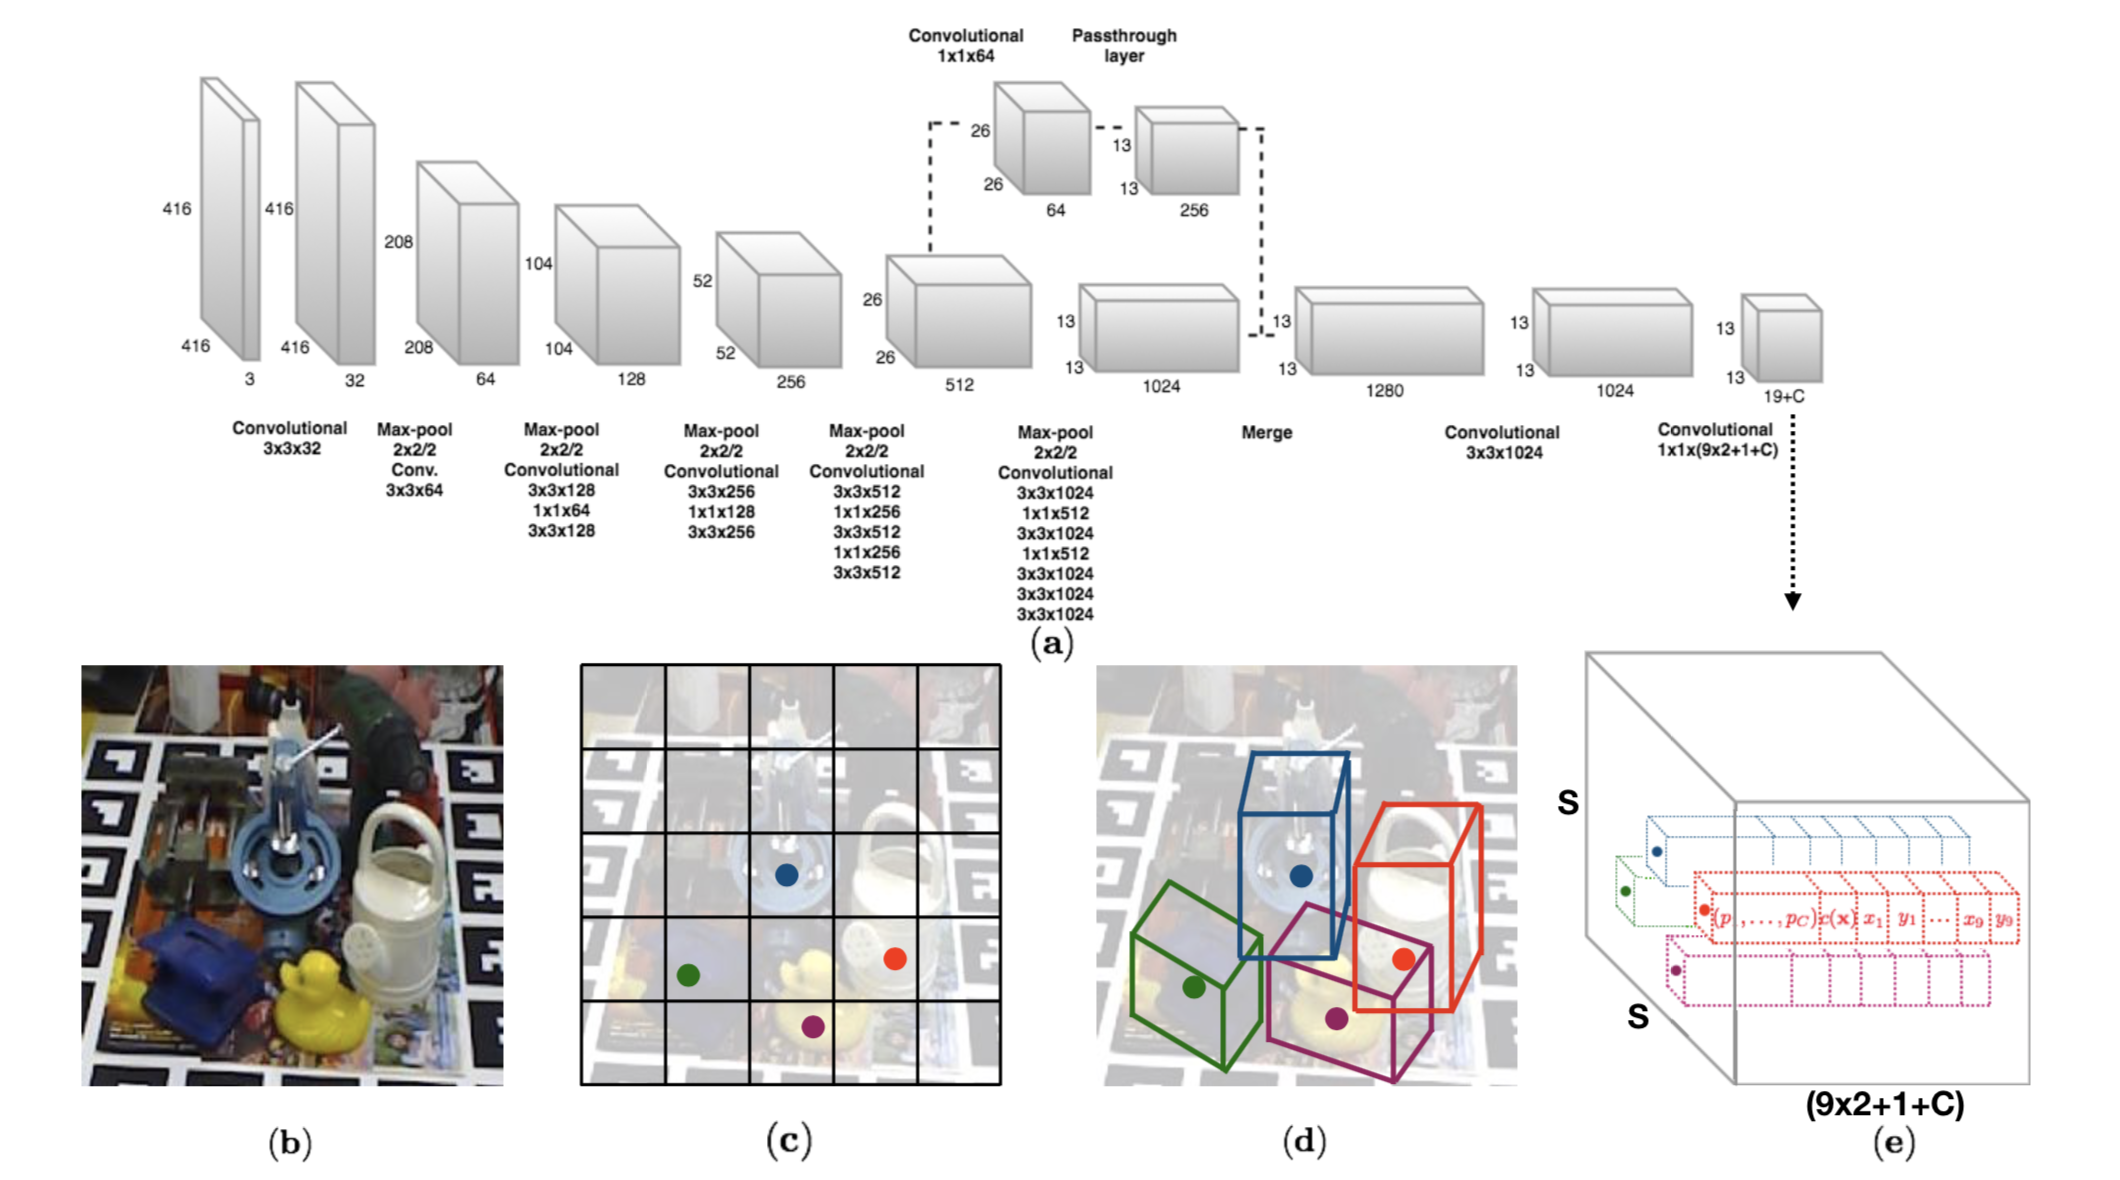
\includegraphics[width=\linewidth]{methodology.png}
  \caption{Network architecture from \cite{tekin2018real}: (a) The proposed CNN architecture. (b) An example input image with four objects. (c) The $S \times S$ grid showing cells responsible for detecting the four objects. (d) Each cell predicts 2D locations of the corners of the projected 3D bounding boxes in the image. (e) The 3D output tensor from our network, which represents for each cell a vector consisting of the 2D corner locations, the class probabilities and a confidence value associated with the prediction.}
  \label{fig:methodology}
\end{figure}

Our model follows B. Tekin's model \cite{tekin2018real} which performs 6D object pose detection based on YOLO v2 architecture. Since YOLO's network is designed to regress only 2D bounding boxes, a few more 2D points had to be added for 6D object detection. In our model, a CNN-based network predicts 2D projections of the corners of the 3D bounding box around the object. Then a PnP algorithm is used to compute camera pose efficiently given the 2D coordinates and 3D ground control points for the bounding box corners.

We choose the keypoints of the 3D object model as the 8 corners of the object's tight 3D bounding box plus the centroid of the object's 3D model. Thus, we parameterize the 3D model of each object with 9 control points. The control points are guaranteed to be well spread out in the 2D image. In practice, the control points can be defined in other ways as well.

Given a single full color image as input, our model processes it with a fully convolutional architecture and divides the image into a 2D regular grid containing $ S \times S $ cells as YOLO does. Each grid is associated with a multidimensional vector as the output. The vector consists of the predicted locations of the 9 control points, C class probabilities of the object and one overall confidence score. Thus, the output of our network is a 3D sensor of size $ S \times S \times D $. In out case, $D = 9\times2+1+C$, where the location of each 2D control point contain 2 coordinates and C is the number of classes. Same as YOLO, the conditional class probabilities is  conditioned on the cell containing an object. The network is based on YOLO v2's network and consists of 23 convolutional layers and 5 max-pooling layers.

\begin{figure}
\centering
  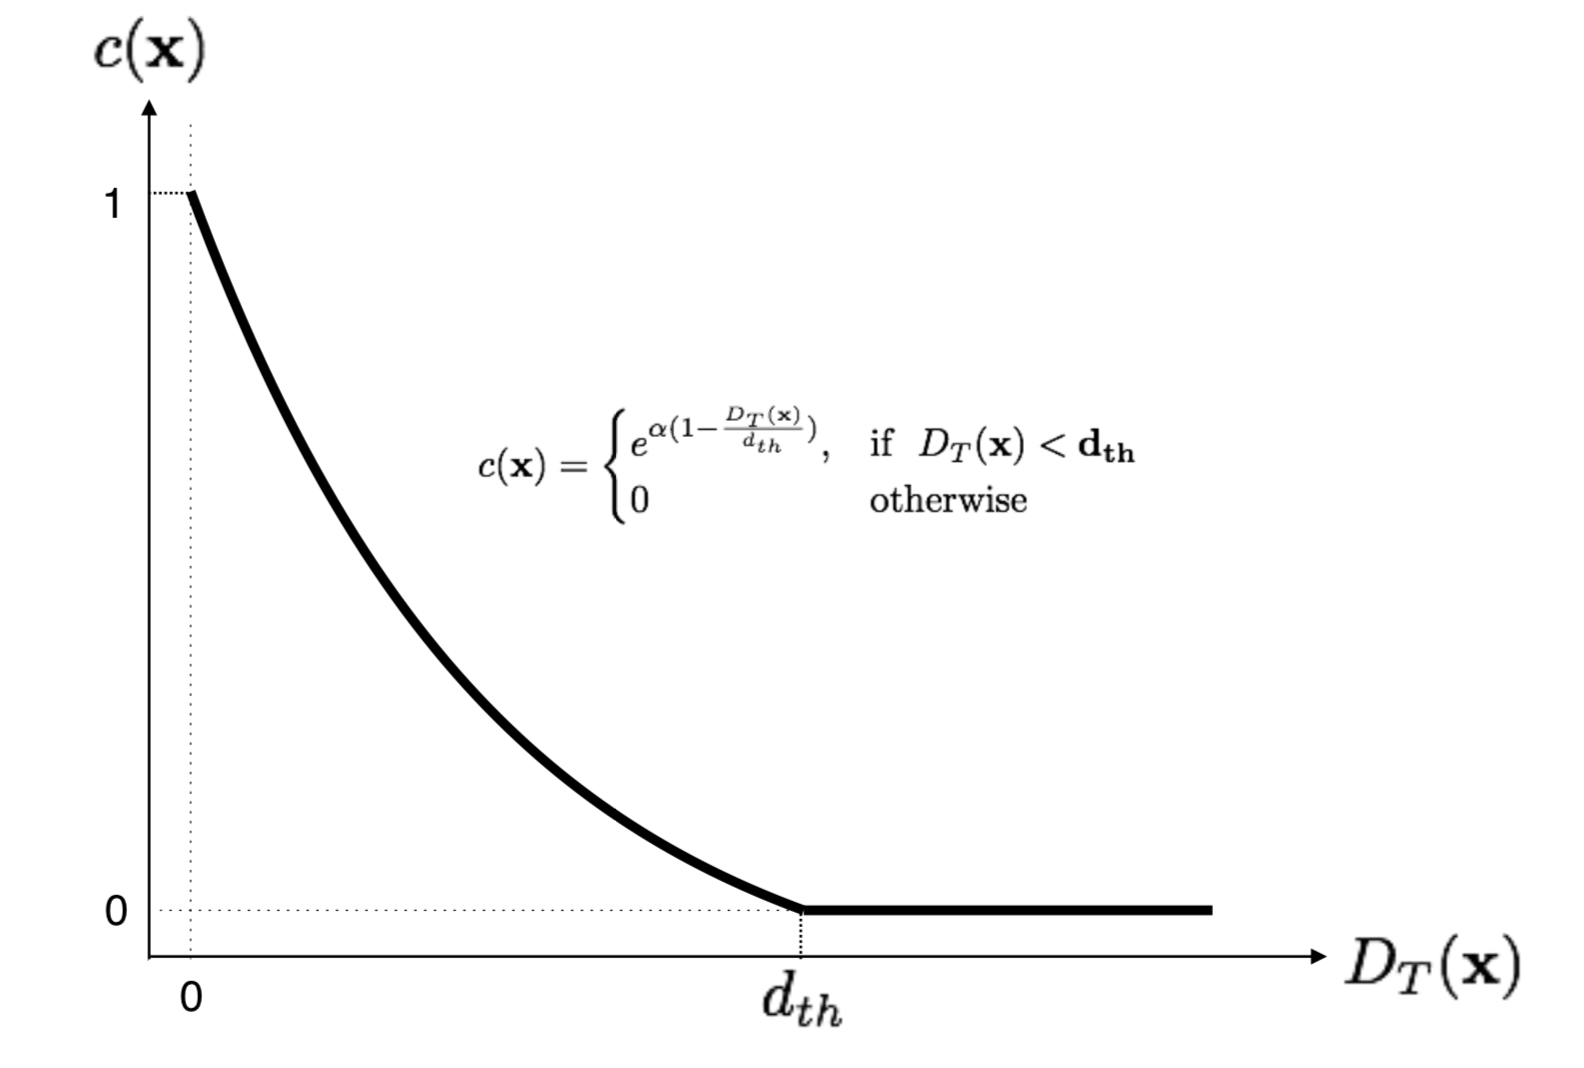
\includegraphics[width=0.6\linewidth]{conf_func.png}
  \caption{Confidence function}
  \label{fig:conf_func}
\end{figure}
In YOLO the confidence value is calculated by the intersection over union (IOU) between the predicted box and the ground truth. However, we have 3D objects in our case and it is not easy or fast to calculate the IOU over 3D voxel cuboids. In order not to slow down the training procedure, we take a confidence function to model the confidence value as introduced in \cite{tekin2018real}. As shown in figure , the confidence function c(x) returns a confidence value for a predicted 2D point, denoted as x, based on its distance $ D_{T}(x) $ from the ground truth 2D point. Formally, the confidence function is defined as follows:
\begin{equation}
\label{eqn:conf_func}
c(x)=\left\{
\begin{aligned}
&e^{\alpha(1-\dfrac{D_{T}(x)}{d_{th}})}, &\text{if } D_{T}(x) < d_{th}\\
&0 &\text{otherwise}
\end{aligned}
\right.
\end{equation}
where $ D_{T}(x) $ is the euclidean distance in the image space, $ d_{th} $ is a cut-off value $ d_{th} $ so that if the distance is not less than it, simply set the confidence score to 0, and the parameter $ \alpha $ defines the sharpness of the exponential function. The overall confidence score of the predicted bounding box is then computed as the mean value of the confidence value of all the control points.

\section{Training}
During training the confidence value is computed on the fly using the confidence function in Eq. \ref{eqn:conf_func} to measure the distance between the current coordinates prediction and the ground truth, DT(x)
Predict the offsets for the 2D coordinates with respect to (cx, cy), the top-left corner of the associated grid cell.
We constrain the centroid within the associated grid cell, i.e. the offset of the centroid to lie between 0 and 1. For the corner points we do not constrain the network’s output as those points should be allowed to fall outside the cell.

\section{Prediction}
Predictions at cells with low confidence values will be pruned.

\section{Implementation Details}

We train our network on Leonhard cluster. Since we have limited memory assigned to each GPU node  on the cluster, we can only train with batch size of 8.
700 epochs
Learning algorithm
-SGD
-Adam
Error metric
-Error of corner indices ordering
-Unit

